\scanpage{92}
\[
\begin{aligned}
\deleted{\rho}\unsure{\varepsilon|\xi}_1:\quad
 (\unsure{h|\ell}_0,h_1,\underset{\substack{\rotatebox{90}{$=$}\\h_1^{-1}h_0^{-1}}}{h_2})
 &\longmapsto (h_0^{-1},h_1,h_1^{-1}h_0=h_2h_0^2)\\
\deleted{\rho}\varepsilon_2:\quad(h_0,h_1,h_2)&\mathrel{\mapstochar\relbar}(h_0,h_1^{-1},h_1h_0^{-1}=h_1^2h_2)\\
\deleted{\rho}\varepsilon'_1:\quad(h_0,h_1,h_2)&\mathrel{\mapstochar\relbar}(h_{2}^{-1}h_1,h_1^{-1},h_2)=\\
\varepsilon'_2&\\
\deleted{\rho}\varepsilon''_1&\\
\deleted{\rho}\varepsilon''_2:\quad(h_0,h_1,h_2)&\longmapsto(h_0^{-1},h_0h_2^{-1},h_2^{\deleted{\unsure{+1|-1}}})
\end{aligned}
\]

\[
\begin{aligned}
\rho_1=\deleted{\rho}\varepsilon_1\deleted{\rho}\varepsilon''_2:\qquad
 h_0&\longmapsto h_0^{-1}\mathrel{\mapstochar\relbar}h_0\\
 h_1&\longmapsto h_0h_2^{-1}\longmapsto h_0^{-1}h_0^{-1}h_1=h_0^{-2}h_1\\
 h_2&\mathrel{\mapstochar\relbar}h_2\longmapsto h_1^{-1}h_0=h_2h_0^2\\
{\deleted{\rho}\varepsilon''_2}^{-1}\deleted{\rho}\varepsilon_1^{-1}:\qquad
 h_0&\mathrel{\mapstochar\relbar}\unsure{h^{-1}|h_0^{-1}|\ell_0^{-1}}\mathbin{\text{---}}h_0\\
 h_1&\longmapsto h_1\mathrel{\mapstochar\relbar}h_0h_2^{-1}=h_{\unsure{0}}^2h_1\\
 h_2&\mathrel{\mapstochar\relbar}h_1^{-1}h_0\longrightarrow h_2^{\deleted{\unsure{-1}}}h_0^{-1}h_0^{-1}=h_2h_0^{-2}
\end{aligned}
\]
\[
(\rho_1\rho''_2)^2\qquad\qquad\qquad x,
\]
\diagram{\begin{tikzcd}[ampersand replacement=\&,column sep=small,row sep=small]
\mathbb Z^3\arrow[r]\&\mathbb Z^3\arrow[r]\&\mathbb Z\\
\mathbb Z\arrow[u]\&V(\mathbb Z)\&
\end{tikzcd}}
\[
\begin{aligned}
(x_0\ x_1\ x_2)&\longrightarrow(-x_0,x_1,x_0-x_1)\\
 e_0\quad e_1\quad e_2&\\
 e_1-e_0,\ e_2-e_0&
\end{aligned}
\]
\figure{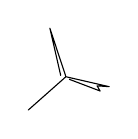
\begin{tikzpicture}[scale=.55,line cap=round,line join=round]
\draw (0,0)--(-.87,-.77) (0,0)--(-.37,1.12)--(-.12,.03) (0,0)--(1,-.23)--(.72,-.21)--(.79,-.33)--(.08,-.06);
\end{tikzpicture}}
\[
e_2=-e_0-e_1
\]
\diagram{\begin{tikzcd}[ampersand replacement=\&,column sep=small,row sep=tiny]
\deleted{\unsure{x+{}}}\mathbb Z\arrow[r]\&\mathbb Z^3\arrow[r,dash]\&\mathbb Z^3\\
\&e_{\unsure{1}}\arrow[r]\&e_{2}-e_3\\
\&e_2\arrow[r]\&{}
\end{tikzcd}}
\[
V^{\mathrm I}
\]
\[
\begin{aligned}
\deleted{(x,y,\unsure{z})}\quad\big[\, (e_0,e_1,e_2)&\longrightarrow(-e_0,e_1;e_0-e_1)\\
 (e_1,e_2,e_3)&\longrightarrow(e_0,-e_1\unsure{;|)}e_1-e_0)\\[2pt]
\big[\, (e_0,e_1,e_2)&\longmapsto(2e_1+e_0,-e_1\deleted{\unsure{)}};e_2\\
 (e_0,e_1,e_2)&\longmapsto\boxed{(-e_0-2e_1,\ e_1};-e_2)\\[2pt]
\big[\, [e_0,e_1,e_2)&\longmapsto\boxed{(e_0,\unsure{-2e_0-e_1}};-e_2)\\
 (e_0,e_1,e_2)&\longmapsto(-e_0,\unsure{2e_0+e_1},e_2)
\end{aligned}
\]
% archive sheet number: 91
